\documentclass[12pt]{article}
\usepackage[a4paper, total={6in, 8.5in}]{geometry}
\usepackage[final]{graphicx}
\usepackage{amsmath}
\usepackage{amssymb}
\usepackage{minted}
\usepackage{multicol}
\usepackage{subcaption}
\usepackage{tabularx}
\usepackage[english]{babel}

\title{Constructing of three phase transformer using three single phase transformers
\& observing line \& phase voltage relation in primary and
secondary windings.}
\author{}
\date{}

\begin{document}
\vspace*{\fill}
\begin{center}

    \emph{Heaven's Light is Our Guide} \\
    \textbf{Rajshahi Universiy of Engineering and Technology} \\

    \begin{figure}[h]
        \centering
        
\includegraphics[scale=.34]{images/RUET_logo.png}
        \label{fig:ruet_logo}
    \end{figure}
    \vspace{5mm}

    \textbf{Course Code}\\
    ECE 2208\\
    \vspace{3mm}
    \textbf{Course Title}\\
    Electrical Machines - I Sessional

    \vspace{5mm}
    \textbf{Experiment Date:} {October 4, 2023,}\\
    \textbf{Submission Date:} {October 18, 2023}\\

    \vspace{5mm}
    \textbf{Lab Report 1:} Polarity test of a transformer.\\

    \vspace{15mm}

    \begin{tabular}{c|c}
        \textbf{Submitted to} & \textbf{Submitted by} \\
        Md. Omaer Faruq Goni  & Md. Tajim An Noor     \\
        Lecturer              & Roll: 2010025         \\
        Dept of ECE, RUET     &                       \\
    \end{tabular}

\end{center}
\vspace*{\fill}

\pagebreak

\maketitle
\section{Introduction}
\subsection*{Three phase transformer}
To construct a three phase transformer, three single-phase transformers can be connected. Alternatively, a pre-assembled and balanced three-phase transformer consisting of three pairs of single-phase windings mounted onto a single laminated core can be used. This is also known as a 3-$\Phi$ transformer.\\\\
The primary and secondary windings of a transformer can be connected in different configuration to meet practically any requirement. In the case of three phase transformer windings, two forms of connection are: “Star” (wye) \& “delta” (mesh).\\\\
The combinations of the three windings may be with the primary $\Delta$-connected and the secondary Y-connected, or Y-$\Delta$, $\Delta$-$\Delta$, Y-Y depending on the transformers use. When transformers are used to provide three or more phases they are generally referred to as a Polyphase Transformer.\cite{trans}


\pagebreak
\subsection*{Circuit Diagrams}
\begin{figure}[htbp!]
    \centering
    % 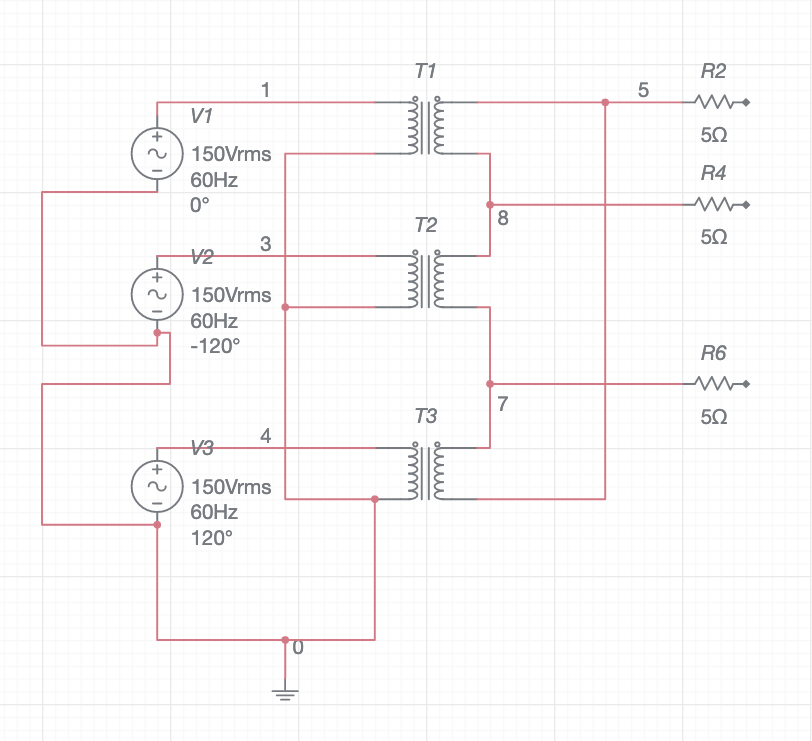
\includegraphics[width=.8\linewidth]{images/output/ydel.png}
    \caption{Circuit diagrams for Y-$\Delta$ three transformer connection.}
    \label{fig:fig}
\end{figure}
\vspace{\fill}

\section{Tools Used}
\begin{itemize}
    \item Single Phase Transformer (150V - 1A), 3 pieces
    \item Connecting wires
    \item Ammeter (0A - 5A)
    \item Voltmeter (0V - 120V)
    \item Wattmeter
    \item Three Phase AC supply (220V)
    \item Three phase Variac (0-250V)
\end{itemize}

\section{Data \& Calculation}
\subsection{Data Table:}
\begin{table}[H]
    \centering
    \caption{Y Connection}
    \begin{tabular}{|c|c|c|c|c|c|}
        \hline
        \bf{V\textsubscript{an}} & \bf{V\textsubscript{bn}} & \bf{V\textsubscript{cn}} & \bf{V\textsubscript{AB}} & \bf{V\textsubscript{BC}} & \bf{V\textsubscript{CA}} \\
        \hline
        100.8                    & 100.7                    & 101.5                    & 175.8                    & 176.8                    & 177.4                    \\
        \hline
    \end{tabular}
\end{table}
\begin{table}[H]
    \centering
    \caption{$\Delta$ Connection}
    \begin{tabular}{|c|c|}
        \hline
        \bf{V\textsubscript{an}} & \bf{V\textsubscript{AB}} \\
        \hline
        150.6                    & 131.7                    \\
        \hline
    \end{tabular}
\end{table}

\subsection{Calculation:}
For Y-connection, \[V_L = \sqrt{3}V_P\] \\
Line Voltage, \[V_{an} = 100.8V\] \\
$\therefore$ Phase voltage, \[V_{AB} = \sqrt{3}\times 100.8 = 174.59\] \\
Average Measured phase voltage, \[V_{AB} = \frac{175.8+176.8+177.4}{3} = 176.67V\] \\\\
For $\Delta$-connection, \[V_L = V_P\] \\
Line voltage, \[V_{an} = 100.7V\] \\
Measured phase voltage, \[V_{AB} = 100.7V\] \\

\section{Discussion}
Just like three phase supply, in transformers, the relation persists. In wye connection, the line \& phase voltages aren't the same but in delta connection, they are the same.


\section{Conclusion}
Since this experiment was done with AC supply, utmost caution was exercised to avoid any accident. Additionally, the line and phase current relation wasn't tested as it'd require precise and cautious connection. To avoid any dangers, only the voltage relation was done in this experiment.
\bibliographystyle{IEEEtran}
\bibliography{ref}

\end{document}